
\documentclass[10pt]{article}
\usepackage[utf8]{inputenc}
\usepackage[spanish]{babel}
\usepackage{authblk}
\usepackage{amsmath}
\usepackage{graphicx}
\usepackage{booktabs}
%\usepackage{hyperref}
%\usepackage{bookmark}
% Título del Trabajo Práctico
\title{Sistema Multi-Agente para la Gestión y Optimización de Carteras de Inversión en Renta Variable}

\author[1]{José Carlos Carbone}
\author[1]{Marco Sebastián Padilla}
\author[1]{Nilayvi Stephani Barrientos Pérez}
\author[1]{Federico Hernan Sanches}
\affil[1]{Maestría en Inteligencia Artificial}

\date{Marzo 2026}



\begin{document}

\maketitle

\begin{abstract}
Este trabajo presenta el diseño e implementación de un asistente financiero inteligente basado en una arquitectura de micro-agentes coordinados. El sistema integra datos en tiempo real de activos de renta variable (Acciones), permitiendo al usuario final interactuar mediante lenguaje natural a través de la plataforma Telegram. La solución no solo centraliza la visualización del portfolio, sino que aplica modelos de optimización de máximo ratio de Sharpe, análisis de sentimiento de noticias y simulaciones estocásticas para proyectar flujos de fondos y proponer rebalanceos estratégicos.
\end{abstract}

\section{Introducción}
El acceso a mercados financieros ha crecido exponencialmente, sin embargo, la complejidad técnica para analizar acciones locales e internacionales sigue siendo una barrera para el inversor promedio. Este proyecto propone un asistente que utiliza Modelos de Lenguaje de Gran Escala (LLM) no solo como interfaz, sino como orquestador de herramientas cuantitativas.

El objetivo principal es resolver la asimetría de información mediante tres pilares:
\begin{itemize}
    \item \textbf{Retrospectiva:} Análisis de costo de oportunidad frente a benchmarks.
    \item \textbf{Proyección:} Estimación de flujos futuros y volatilidad.
    \item \textbf{Optimización:} Sugerencia de carteras eficientes basadas en el perfil de riesgo.
\end{itemize}

\section{Arquitectura del Sistema}
Se ha optado por una arquitectura de \textit{Sistema Multi-Agente} (MAS) implementada mediante el framework \textit{LangGraph}. Esta decisión permite desacoplar la lógica de negocio de la obtención de datos y el procesamiento de lenguaje natural.

\begin{figure}[h] % [h] intenta ponerla 'here' (aquí)
    \centering
    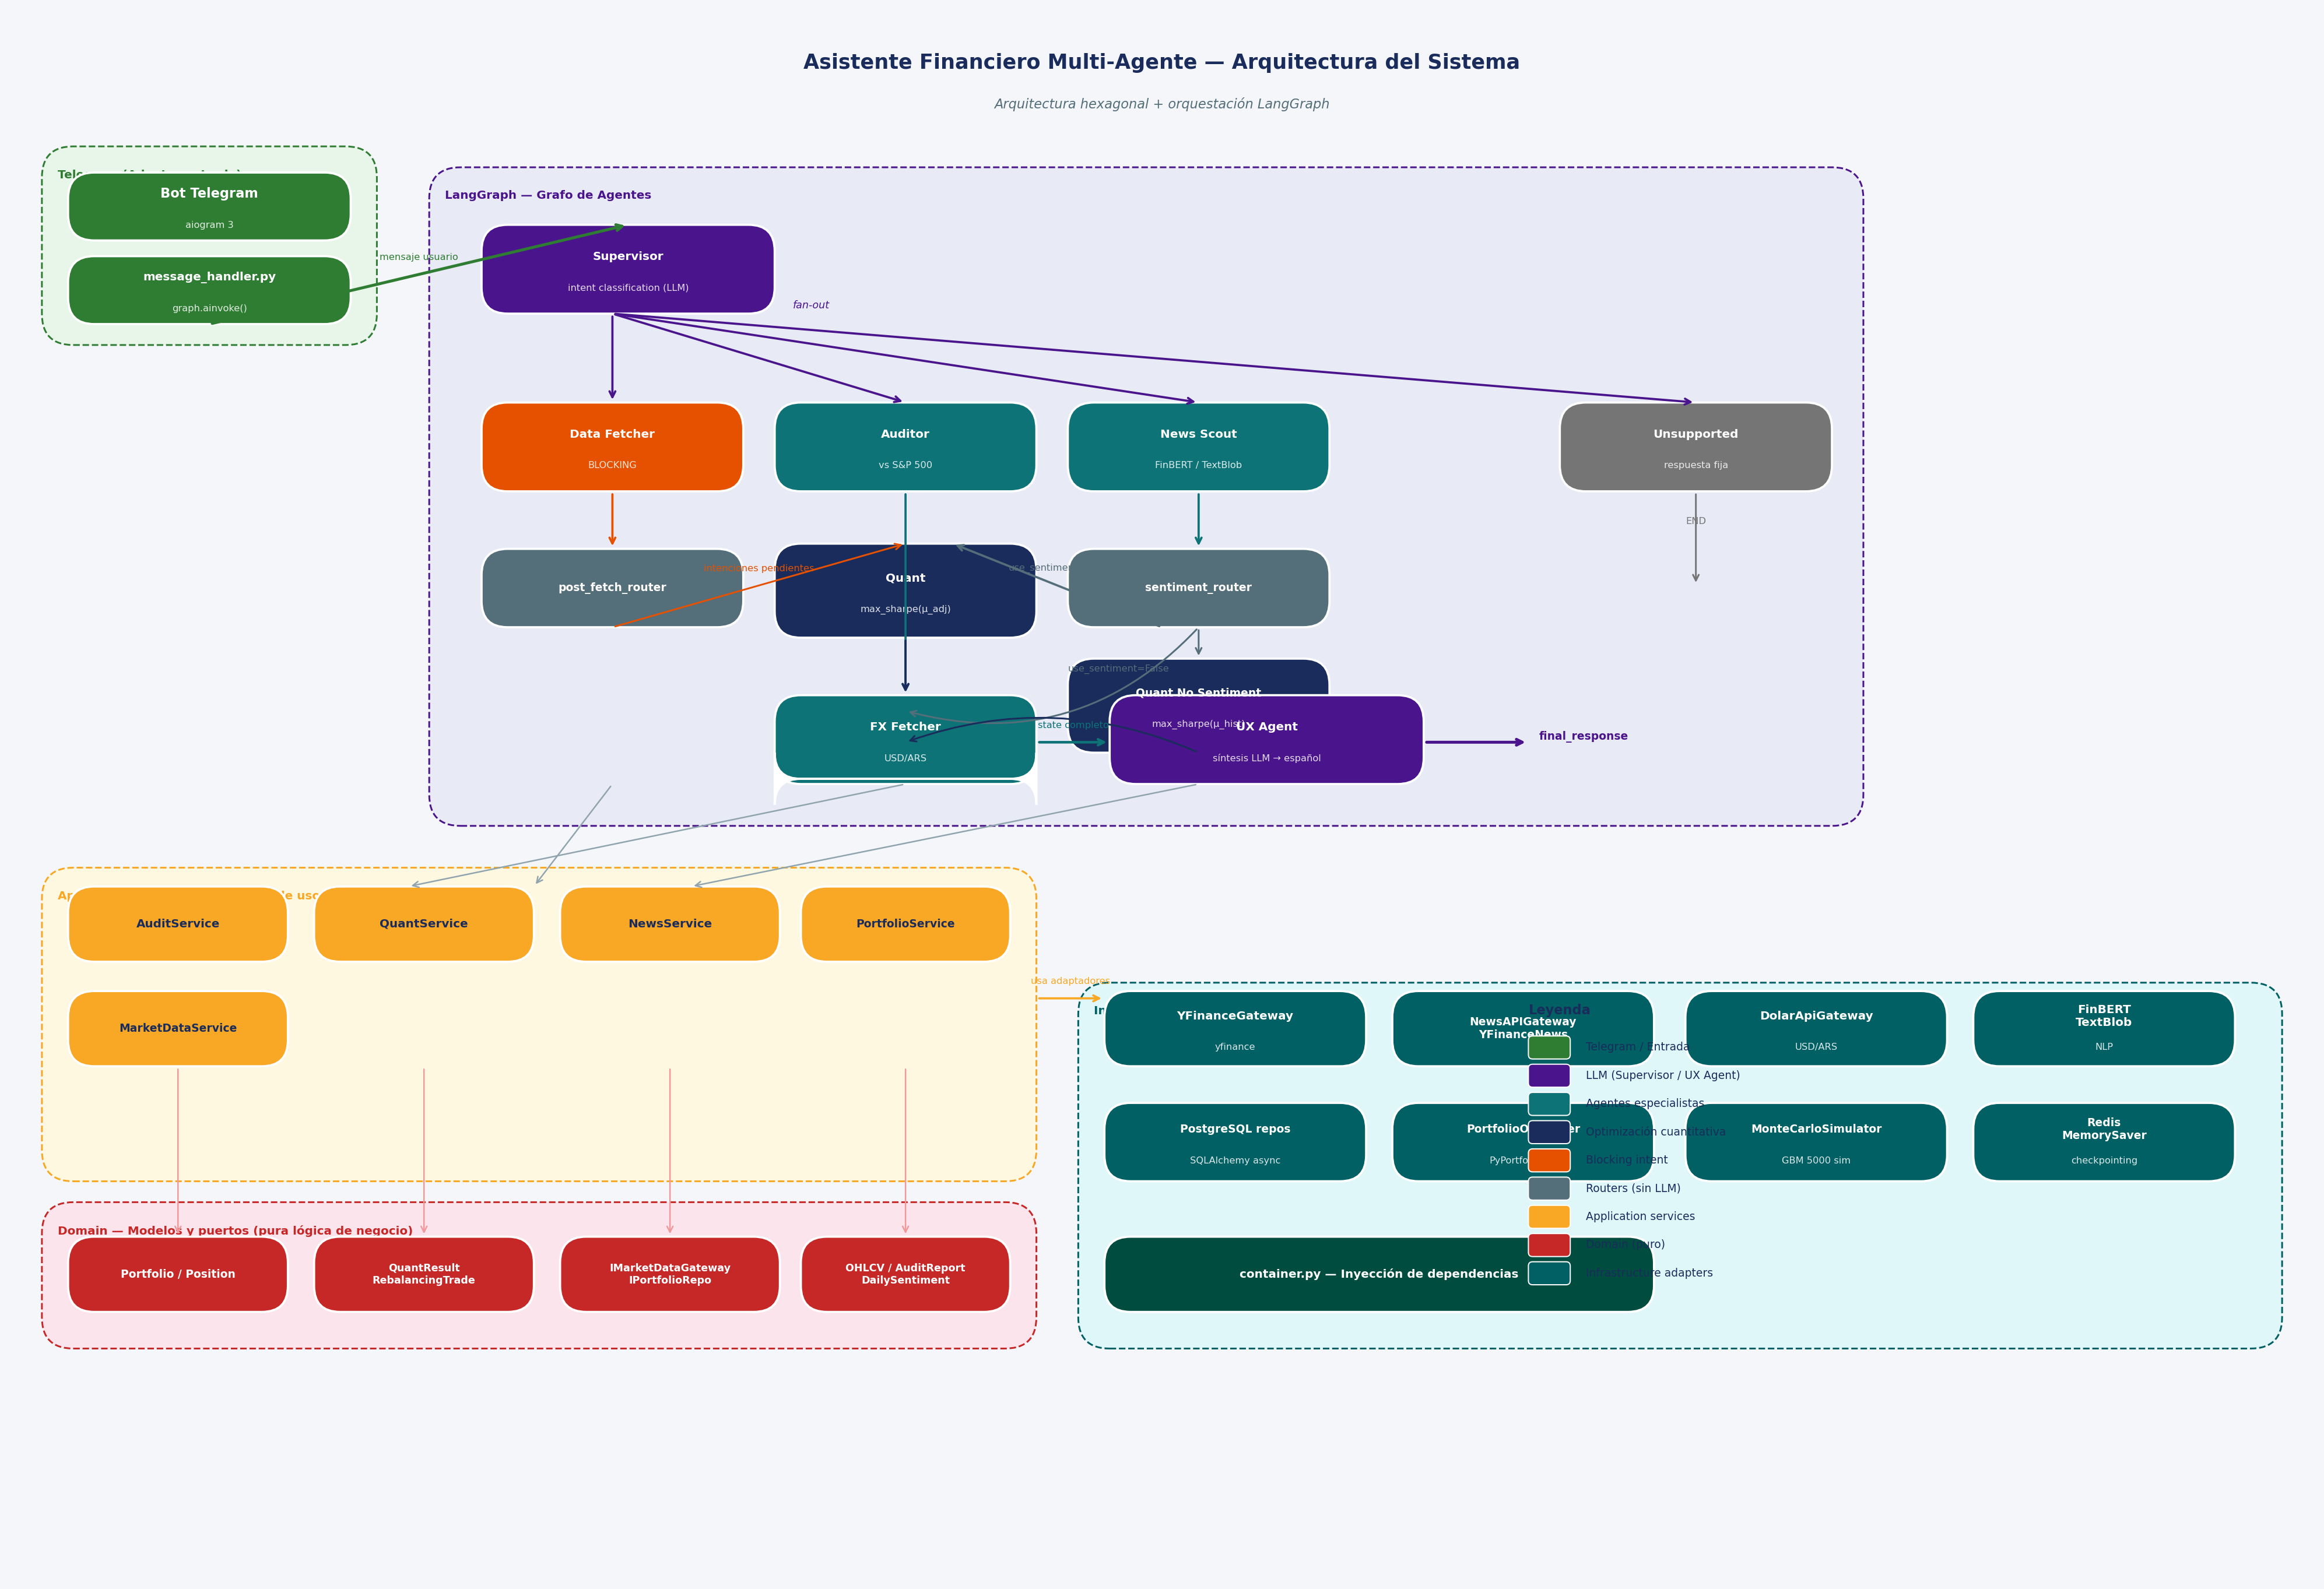
\includegraphics[width=\linewidth]{arquitectura_asistente}
    \caption{Arquitectura del Sistema Multi-Agente propuesto.}
    \label{fig:arquitectura}
\end{figure}

\subsection{Agente Orquestador (The Supervisor)}
Actúa como el nodo central de decisión. Utiliza \textit{Function Calling} para clasificar la intención del usuario y dirigir el flujo hacia los agentes especialistas.

\subsection{Agentes Especialistas}
\begin{enumerate}
    \item \textbf{Data Fetcher:} Encargado de la persistencia en PostgreSQL y la ingesta de datos vía APIs (yfinance). Es el único agente \textit{blocking}: cuando se combina con otras intenciones, corre primero y el \textit{post\_fetch\_router} despacha los especialistas restantes una vez que los datos están disponibles.
    \item \textbf{The Auditor:} Calcula el rendimiento histórico comparado con el Dólar MEP y el índice S\&P 500.
    \item \textbf{The Quant:} El motor matemático. Utiliza la librería \textit{PyPortfolioOpt} para maximizar el ratio de Sharpe y modelos de Monte Carlo (GBM) para proyecciones de flujos futuros. Cuando el sentimiento está activo, corre en paralelo con \textbf{Quant No Sentiment} para comparar ambas optimizaciones.
    \item \textbf{Quant No Sentiment:} Instancia paralela del agente Quant que opera con retornos históricos puros, sin ajuste de sentimiento. Permite al usuario comparar el impacto del sentimiento sobre los pesos óptimos bajo el mismo criterio de optimización.
    \item \textbf{The News Scout:} Implementa análisis de sentimiento sobre noticias financieras de última hora usando FinBERT o TextBlob. Alimenta al agente Quant con los scores de sentimiento por ticker.
    \item \textbf{FX Fetcher:} Obtiene el tipo de cambio USD/ARS actualizado para contextualizar los resultados en moneda local.
    \item \textbf{UX Agent:} Sintetiza los resultados de todos los agentes especialistas en una respuesta en español comprensible para el usuario final.
\end{enumerate}

\section{Metodología de Optimización}
Para la optimización de la cartera, el sistema se basa en la teoría moderna de selección de cartera (Markowitz). Dado un conjunto de activos con retornos esperados $\mu$ y una matriz de covarianza $\Sigma$, se busca el portfolio tangente que maximiza el ratio de Sharpe:

$$ \max \frac{w^T \mu - r_f}{\sqrt{w^T \Sigma w}} $$

Sujeto a:
$$ \sum w_i = 1, \quad w_i \geq 0 $$

donde $r_f$ es la tasa libre de riesgo (5\% anual por defecto). Este portfolio se ubica en el punto de tangencia entre la \textit{Capital Market Line} (CML) y la frontera eficiente.

El sistema ejecuta esta optimización en dos variantes en paralelo: una con $\mu$ ajustado por sentimiento ($\mu_{adj}$) y otra con $\mu$ histórico puro. Al utilizar el mismo criterio de optimización en ambos casos, la diferencia en los pesos resultantes es atribuible exclusivamente al ajuste de sentimiento, haciendo la comparación directamente interpretable.


\section{Sinergia Multi-Agente: News Scout y Optimización Quant}
La innovación de este sistema radica en la retroalimentación entre el análisis cualitativo y el cuantitativo. Mientras que el \textit{Agente Quant} opera sobre series de tiempo históricas para calcular la matriz de covarianza $\Sigma$, el \textit{News Scout} proporciona un "ajuste de sentimiento" ($\alpha_{sent}$) que modifica los retornos esperados en tiempo real.

El modelo de retorno ajustado se define como:
\[ E[R_{adj}] = E[R_{hist}] \cdot (1 + \lambda \cdot s) \]
Donde $s \in [-1, 1]$ es el score de sentimiento derivado del procesamiento de lenguaje natural (NLP) de noticias financieras y $\lambda$ es un factor de sensibilidad al mercado. Esta integración permite que el sistema detecte eventos de ``cisne negro'' o noticias corporativas críticas antes de que se reflejen plenamente en el precio histórico. La ejecución paralela de ambas variantes (con y sin sentimiento) expone al usuario la diferencia concreta en pesos y ratio de Sharpe, cuantificando el valor informativo del análisis de sentimiento.

\section{Desarrollo Técnico}
El stack tecnológico seleccionado comprende Python 3.11+, utilizando \textit{Aiogram} para la interfaz de Telegram y \textit{OpenAI/Anthropic} como modelos de razonamiento. La integración de los agentes se realiza mediante grafos dirigidos acíclicos (DAG), garantizando que la respuesta final sea sintetizada por un agente de UX que traduce métricas complejas a un lenguaje comprensible.

\section{Resultados esperados/Conclusión}
La implementación de un sistema multi-agente permite una escalabilidad superior a los chatbots lineales tradicionales. La capacidad de integrar análisis de noticias con modelos econométricos tradicionales posiciona a este asistente como una herramienta integral para la toma de decisiones financieras en tiempo real.


\end{document}